\documentclass{article}
\usepackage{graphicx}
\usepackage[style=ieee]{biblatex} % Establecer el estilo de las referencias como IEEE
\usepackage{xcolor}
\usepackage{hyperref}
\usepackage{titletoc}
\usepackage{adjustbox}
\usepackage{amsmath} 
\usepackage[spanish]{babel}

\usepackage{listings}
\hypersetup{
    colorlinks=true,
    linkcolor=blue, % Color del texto del enlace
    urlcolor=blue % Color del enlace
}

\usepackage{longtable} % Agrega el paquete longtable

\definecolor{mygreen}{RGB}{0,128,0}

\usepackage{array} % Para personalizar la tabla
\usepackage{booktabs} % Para líneas horizontales de mejor calidad
\usepackage{graphicx} % Paquete para incluir imágenes
\usepackage{float}

% Definir márgenes
\usepackage[margin=1in]{geometry}

\renewcommand{\contentsname}{\textcolor{mygreen}{Tabla de Contenidos}}

\begin{document}

\begin{titlepage}
    \centering
    % Logo de la Universidad
    
\includegraphics[width=0.48\textwidth]{logo_universidad.png}
    \par\vspace{2cm}

    % Nombre de la Universidad y detalles del curso
    {\Large \textbf{Universidad Nacional de Colombia} \par}
    \vspace{0.5cm}
    {\large Ingeniería de Sistemas y Computación \par}
    {\large 2025969 Modelos estocásticos y simulación en computación y comunicaciones (01)\par}
    \vspace{3cm}

    % Detalles del laboratorio y actividad
    {\large \textbf{Taller 1} \par}
    {\large Taller 1 \par}
    \vspace{3cm}

    % Lista de integrantes
    {\large \textbf{Integrantes:} \par}
    \vspace{0.5cm}
    \begin{tabular}{ll}
    Javier Andrés Tarazona Jiménez & jtarazonaj@unal.edu.co \\
    Jefferson Duvan Ramirez Castañeda & jeramirezca@unal.edu.co \\
    Yenifer Yulieth Mora Segura & ymoras@unal.edu.co \\
    Javier Carrillo & @unal.edu.co \\
    Grevy Joner Rincon Mejia & grrinconm@unal.edu.co \\
    Esteban Carranza & jcarranza@unal.edu.co \\
    Diego & @unal.edu.co \\
    \end{tabular}
    \par\vspace{3cm}

    % Fecha
    {\large Junio 16 de 2025 \par}
\end{titlepage}

\tableofcontents % Inserta la tabla de contenidos

\newpage % Salto de página para separar la tabla de contenidos del contenido del documento

% Contenido del artículo----------------------------------------------------------

%---------------------------------------------------------------------------------
% Intro --------------------------------------------------------------------------
%---------------------------------------------------------------------------------

\section{Introducción}\label{sec:intr}

En un escenario de extinción de incendios forestales mediante drones cooperativos, la comunicación inalámbrica entre los dispositivos se ve constantemente afectada por obstáculos naturales (árboles, relieve), interferencias y la movilidad dinámica del enjambre. Este trabajo aborda un problema concreto: cuando un dron se desconecta momentáneamente del líder de su grupo (Cluster Head) debido a estas adversidades, pierde capacidad de coordinación crítica para la misión, retrasando la respuesta ante focos de incendio y aumentando el consumo energético por retransmisiones.

Para resolver este desafío operativo, proponemos una solución basada en redes MANET jerárquicas, donde los drones desconectados adoptan temporalmente el rol de líder (CH-temporal). Este enfoque práctico se sustenta en modelos teóricos de movilidad grupal y algoritmos de reclusterización dinámica, evaluando umbrales de desconexión basados en calidad de señal, energía remanente y presencia de obstáculos. La implementación en NS-3 demuestra que este método reduce el tiempo de recuperación de conexiones comparado con protocolos tradicionales, manteniendo la efectividad del enjambre incluso en condiciones adversas.


%---------------------------------------------------------------------------------
% Marco Teórico ------------------------------------------------------------------
%---------------------------------------------------------------------------------

\section{Marco Teórico}\label{sec:marc}

\subsection{Redes MANET}
Las redes móviles ad hoc, conocidas como \textbf{MANET (Mobile Ad Hoc Networks)}, son un tipo de red inalámbrica \textbf{descentralizada} y \textbf{auto-configurable} formada por dispositivos móviles que se comunican entre sí sin requerir una infraestructura fija, como estaciones base o routers cableados. Cada nodo en la red actúa simultáneamente como terminal —que genera y recibe información— y como enrutador, facilitando el envío de datos a través de múltiples saltos (\textit{multihop}) hasta alcanzar su destino. Esta capacidad de autoorganización hace que las MANET sean especialmente útiles en contextos donde no es posible contar con infraestructura tradicional, como en zonas de desastre, operaciones militares, entornos rurales o redes vehiculares dinámicas.

El diseño y funcionamiento de una red MANET implica afrontar múltiples \textbf{desafíos técnicos} derivados principalmente de la \textbf{movilidad constante} de los nodos y la inestabilidad inherente a los enlaces inalámbricos. A diferencia de las redes convencionales, sustentadas en una \textbf{topología fija}, las MANET presentan una \textbf{topología altamente dinámica}, influenciada por el desplazamiento de los nodos, la interferencia del medio de transmisión y las restricciones energéticas. Esta naturaleza cambiante genera complejidades en aspectos críticos como el establecimiento y mantenimiento de rutas eficientes, la gestión del consumo energético, la calidad del servicio (QoS) y la seguridad de las comunicaciones.


\subsubsection{Características de las redes MANET}
Las redes \textbf{MANET} se caracterizan por la \textbf{movilidad continua} de sus nodos, como teléfonos, sensores, drones o vehículos, lo que provoca cambios constantes en la \textbf{topología de la red} durante su operación. Esta movilidad espacial, en dos o tres dimensiones, modifica dinámicamente los enlaces disponibles, ya que la \textbf{conectividad depende del rango de transmisión} entre nodos. Adicionalmente, estas redes se construyen de forma espontánea mediante procesos de \textbf{auto-configuración}, en los que basta con que los nodos compartan protocolos comunes de descubrimiento y enrutamiento para establecer enlaces funcionales. El \textbf{enrutamiento distribuido}, soportado por protocolos como \textbf{AODV}, \textbf{DSR}, \textbf{OLSR}, \textbf{B.A.T.M.A.N.} o \textbf{DYMO}, permite hallar rutas sin necesidad de un nodo central de control. Dado que los nodos pueden no estar siempre en contacto directo, la red opera mediante transmisión \textit{multihop}, en la que los paquetes se reenvían a través de múltiples saltos para alcanzar su destino. Finalmente, las MANET deben enfrentar \textbf{restricciones inherentes de recursos}, como energía limitada, canal inalámbrico compartido y ancho de banda reducido, lo que condiciona el diseño de protocolos eficientes para el acceso al medio, calidad de servicio y seguridad.

A diferencia de las redes inalámbricas tradicionales como las redes celulares o Wi-Fi con infraestructura, las MANET operan bajo principios radicalmente distintos. Mientras que las primeras dependen de \textbf{puntos de acceso fijos} o torres de telecomunicaciones con \textbf{cobertura planificada} y \textbf{gestión centralizada}, las MANET prescinden de infraestructura fija y adoptan una \textbf{gestión distribuida}, en la que cada nodo toma decisiones de enrutamiento de forma autónoma. Esta arquitectura les permite un \textbf{despliegue rápido y flexible}, ideal para entornos impredecibles o de emergencia, aunque con la contrapartida de \textbf{enlaces más inestables} y menor capacidad agregada. Así, mientras las redes tradicionales priorizan \textbf{estabilidad y rendimiento sostenido} a costa de altos costos de infraestructura, las MANET privilegian la \textbf{adaptabilidad} y la \textbf{autonomía} en escenarios dinámicos.



\subsubsection{Aplicaciones de las redes MANET}
Gracias a su \textbf{flexibilidad}, \textbf{autonomía} y \textbf{capacidad de autoorganización}, las redes MANET encuentran aplicación en diversos contextos donde las soluciones de comunicación tradicionales resultan inviables o insuficientes. En el ámbito \textbf{militar}, son fundamentales para establecer comunicaciones tácticas robustas y descentralizadas en entornos hostiles o cambiantes, permitiendo la conectividad entre vehículos, unidades en movimiento y sistemas no tripulados (UAVs). De forma similar, en situaciones de \textbf{emergencia} como terremotos, incendios forestales o inundaciones, estas redes facilitan la coordinación entre equipos de rescate, al permitir el despliegue rápido de enlaces de comunicación en ausencia de infraestructura.

Otras aplicaciones relevantes incluyen la creación de \textbf{redes comunitarias o rurales}, donde los proveedores de servicios de internet (ISP) no tienen presencia y se requiere una solución autosostenible para la conectividad local. En entornos urbanos, las \textbf{redes vehiculares ad hoc (VANET)}, derivadas de la lógica de las MANET, permiten la transmisión de alertas de tráfico y la coordinación entre automóviles para mejorar la seguridad vial. Por último, en escenarios de \textbf{Internet de las Cosas (IoT)}, las MANET sirven como soporte para el monitoreo distribuido de variables ambientales, cultivos o maquinaria en aplicaciones como la \textbf{agricultura de precisión} o la gestión remota de infraestructuras críticas.



\subsection{Jerarquía de Redes MANET}
A medida que las redes MANET crecen en tamaño y complejidad, la gestión descentralizada tradicional comienza a enfrentar serias limitaciones en términos de \textbf{eficiencia}, \textbf{escalabilidad} y \textbf{sobrecarga}. Para abordar estos desafíos, se recurre a la incorporación de \textbf{estructuras jerárquicas} que permiten organizar los nodos en niveles funcionales, como \textbf{clústeres}, \textbf{zonas} o \textbf{dominios}. En este modelo, ciertos nodos asumen roles especializados —como los \textbf{Cluster Heads (CH)} o \textbf{Gateways}— y conforman un \textbf{backbone lógico} encargado de facilitar el control distribuido de la red. Esta organización jerárquica permite \textbf{delegar tareas críticas} de enrutamiento, coordinación y asignación de recursos, lo que reduce la carga global y mejora el rendimiento en entornos altamente dinámicos. Además, al limitar la propagación de paquetes de control a contextos locales, se disminuye significativamente la congestión del canal y se incrementa la eficiencia operativa de la red.


\subsubsection{Arquitectura jerárquica en MANET}
La arquitectura jerárquica en redes MANET introduce un modelo organizativo por niveles que permite mejorar la escalabilidad y reducir la sobrecarga de señalización en entornos altamente dinámicos. A diferencia de las arquitecturas planas, en las cuales todos los nodos comparten responsabilidades similares en el proceso de enrutamiento, una red MANET jerárquica delega ciertas funciones de control y coordinación en nodos especializados, formando una estructura lógica de múltiples capas.

Este tipo de organización se implementa comúnmente a través de mecanismos de \textit{clustering}, donde los nodos se agrupan en dominios o zonas locales. Cada clúster es gestionado por un nodo líder, conocido como \textbf{\textit{Cluster Head} (CH)}, responsable de mantener la conectividad intra-clúster y de actuar como punto de enlace hacia otros clústeres. Sobre esta base, es posible establecer niveles adicionales de jerarquía mediante la inclusión de nodos de mayor rango, o \textit{supernodos}, que se encargan de optimizar la comunicación entre grupos de CH, formando así un \textbf{\textit{backbone}} \textit{multihop} de control.

En términos funcionales, esta jerarquía puede descomponerse en tres niveles principales:
\begin{itemize}
    \item \textbf{Nivel de nodos finales:} compuesto por dispositivos móviles comunes como teléfonos, sensores, vehículos o UAVs, que generan y reciben datos, pero delegan el enrutamiento y la coordinación a nodos superiores.
    \item \textbf{Nivel de clústeres:} donde se agrupan nodos bajo la gestión de un CH, encargado del mantenimiento de rutas locales y de la estabilidad del clúster.
    \item \textbf{Nivel de supernodos o coordinadores interclúster:} responsables de enlazar múltiples clústeres, manejar tráfico agregado y reducir la latencia en trayectos de largo alcance.
\end{itemize}

Este enfoque jerárquico resulta especialmente útil en escenarios complejos como redes tácticas militares, operaciones de búsqueda y rescate, o redes vehiculares distribuidas, donde diferentes grupos de nodos pueden requerir coordinación diferenciada según su ubicación o función operativa.


\subsubsection{Beneficios de la jerarquía en MANET}
La incorporación de una \textbf{estructura jerárquica} en redes MANET aporta ventajas clave en entornos caracterizados por alta movilidad, recursos limitados y necesidad de escalabilidad. Entre los beneficios más relevantes se destacan:

\begin{itemize}
    \item \textbf{Escalabilidad aumentada:} al centralizar parcialmente la toma de decisiones en nodos específicos, se reduce la complejidad del enrutamiento global, lo que permite gestionar un mayor número de nodos sin comprometer la estabilidad de la red.

    \item \textbf{Reducción de la sobrecarga de control:} el tráfico de señalización se limita principalmente al interior de cada clúster, evitando la propagación innecesaria de mensajes de control a través de toda la red y optimizando el uso del \textbf{ancho de banda}.

    \item \textbf{Mejora en la calidad de servicio (QoS):} la jerarquía facilita la aplicación de políticas diferenciadas de tráfico, priorizando flujos críticos como \textbf{voz}, \textbf{video en tiempo real} o datos de sensores, en función de su ubicación dentro de la estructura.

    \item \textbf{Tolerancia a fallos localizada:} la segmentación en clústeres permite aislar errores o desconexiones sin comprometer la totalidad de la red. La pérdida de un nodo o enlace puede ser gestionada de forma local, incrementando la \textbf{robustez} del sistema.

    \item \textbf{Eficiencia energética:} dado que solo los \textbf{Cluster Heads} y enlaces críticos participan activamente en la retransmisión de datos, los nodos ordinarios pueden operar en estados de bajo consumo, prolongando la vida útil de la red en escenarios energéticamente restringidos.

\end{itemize}


\subsubsection{Principales problemas en MANETs jerárquicas de 2 niveles}
La implementación de una arquitectura jerárquica de dos niveles presenta desafíos significativos, entre los cuales destacan los siguientes al modelar o simular redes MANET:

\begin{enumerate}
    \item \textbf{Doble escala mal representada.} 
    En muchos modelos clásicos se asume que todos los nodos tienen un comportamiento homogéneo. Sin embargo, en redes jerárquicas, los \textit{Cluster Heads} (CH) tienden a funcionar como centros de actividad en torno a los cuales se agrupan los nodos miembros. Esta diferencia de roles genera patrones de movilidad no uniformes que no son capturados adecuadamente por modelos planos, lo que lleva a una subestimación de los eventos de reelección de CH y a una sobrevaloración de la estabilidad estructural del \textit{backbone}.

    \item \textbf{Dependencia temporal.} 
    Modelos como \textit{Random Waypoint} tienden a reducir la velocidad promedio de los nodos a largo plazo. En el contexto jerárquico, esto provoca que el nodo líder del clúster parezca detenerse progresivamente, generando enlaces que duran más de lo realista y métricas optimistas de persistencia de ruta y frecuencia de \textit{handoff}.

    \item \textbf{Dependencia espacial y concentración central.} 
    Algunos modelos de movilidad tienden a generar un sesgo hacia el centro del área de simulación, concentrando la presencia de \textit{Cluster Heads} (CH) en esa zona y dejando regiones periféricas con baja densidad. Este desequilibrio produce una topología poco representativa, donde se subestiman los problemas de conectividad en los bordes y se distorsiona el análisis del retardo y la resiliencia del \textit{backbone}.

    \item \textbf{Restricciones geográficas y obstáculos físicos.} 
    En escenarios con edificios, montañas u otras estructuras, los modelos de movilidad con trayectorias fijas como \textit{Pathway} u \textit{Obstacle Mobility} obligan a los clústeres a rodear dichos obstáculos. Esto genera oscilaciones abruptas en la cantidad de saltos entre CH y puede provocar particiones momentáneas de la red, afectando la continuidad del servicio y la estabilidad de las rutas.

    \item \textbf{Limitaciones de los modelos de movilidad grupal.} 
    Modelos como \textit{RPGM} asumen que todos los nodos siguen de forma continua al líder del grupo, sin considerar dinámicas más complejas como divisiones o fusiones entre clústeres. Esta simplificación conlleva una subestimación del tráfico de control necesario para mantener la cohesión del grupo y oculta pérdidas de paquetes que ocurren cuando los nodos se desconectan momentáneamente del clúster.

    \item \textbf{Costos asociados al re-clustering.} 
    Cuando un \textit{Cluster Head} se desplaza rápidamente o pierde conectividad con sus nodos, debe transferir su rol a otro nodo, lo que implica procesos de reelección, resincronización de slots temporales (e.g. TDMA) y actualización de estados. Este comportamiento genera ráfagas de mensajes de control, elevando el consumo energético y el uso del canal en momentos críticos de inestabilidad topológica.

    \item \textbf{Inconsistencias en el direccionamiento jerárquico.} 
    En muchos modelos no se simula el retardo que implica actualizar los prefijos jerárquicos o identificadores de clúster en las tablas de encaminamiento. Durante esta latencia, pueden aparecer retransmisiones innecesarias, rutas erróneas o bucles de reenvío, lo que degrada la eficiencia de la red y la coherencia del plano de control.

    \item \textbf{Interferencia entre enlaces CH y nodos miembros.} 
    Dado que el canal de comunicación es compartido, los enlaces entre \textit{Cluster Heads} y los flujos intra-clúster pueden interferirse mutuamente, especialmente cuando dos clústeres se solapan geográficamente. Esto genera colisiones, pérdidas de paquetes y disminución en la tasa de entrega y el \textit{throughput}, afectando el rendimiento global si no se simula la coordinación inter-clúster.

    \item \textbf{Problemas de escalabilidad del escenario.} 
    En áreas pequeñas, los clústeres tienden a rebotar en los límites del entorno simulado, generando patrones artificiales de movimiento. En cambio, en áreas demasiado grandes, pueden aparecer vacíos entre los CH y los nodos, provocando aislamiento temporal. Estas variaciones hacen que los resultados obtenidos sean altamente sensibles al tamaño del escenario, dificultando su extrapolación a redes reales.

    \item \textbf{Ausencia de trazas jerárquicas reales.} 
    La mayoría de conjuntos de datos disponibles públicamente para simulaciones están basados en redes planas, como movimientos individuales de vehículos o peatones. Esto obliga a parametrizar las simulaciones jerárquicas de forma arbitraria, reduciendo la reproducibilidad de los experimentos y dificultando las comparaciones justas entre diferentes protocolos de enrutamiento jerárquico.

\end{enumerate}


\subsubsection{Comunicación intra-clúster e inter-clúster}

En el contexto de una \textbf{red MANET jerárquica}, el modelo de comunicación se organiza en dos planos complementarios que responden a la segmentación lógica de la red: la \textbf{comunicación intra-clúster} y la \textbf{comunicación inter-clúster}. Cada uno presenta características particulares en términos de alcance, complejidad y gestión de recursos.

\begin{itemize}
    \item \textbf{Comunicación intra-clúster:} se refiere al intercambio de datos dentro de un mismo clúster, donde los nodos seguidores se conectan de forma directa o indirecta con su respectivo \textit{Cluster Head} (\textbf{CH}). Este nodo central coordina el acceso al canal y puede aplicar esquemas de control eficientes, como \textbf{TDMA} o protocolos de \textbf{prioridad adaptativa}, con el fin de evitar colisiones y optimizar la transmisión local. Una herramienta clave para mantener esta organización es el uso de \textbf{beacons}, pequeños paquetes de control que el \textbf{CH} emite periódicamente para anunciar su presencia y permitir que los nodos seguidores verifiquen la conectividad. Estos \textbf{beacons} son esenciales para la \textbf{sincronización} del clúster, la \textbf{detección de eventos de desacoplamiento} y la \textbf{gestión dinámica de enlaces} en escenarios de alta movilidad. Esta centralización parcial reduce la \textbf{interferencia entre nodos} y mejora el rendimiento en aspectos como la \textbf{sincronización}, el \textbf{balanceo de carga} y el \textbf{mantenimiento de rutas estables y cortas}.

    \item \textbf{Comunicación inter-clúster:} comprende los flujos de información entre diferentes clústeres, y es gestionada principalmente por los propios \textbf{Cluster Heads} o por nodos designados como \textbf{gateways}. Estos nodos actúan como puentes entre dominios lógicos y emplean \textbf{protocolos de enrutamiento jerárquico} para mantener la conectividad global. La construcción de rutas entre clústeres puede apoyarse en mecanismos de agregación de información topológica parcial, lo cual permite reducir la \textbf{sobrecarga de señalización} y minimizar la \textbf{latencia}, especialmente en entornos con alta movilidad o distribución desigual de nodos.
\end{itemize}

La coexistencia de estos dos niveles de comunicación permite a la red adaptarse de forma más eficaz a entornos cambiantes, especialmente en escenarios donde se requiere coordinación entre múltiples grupos móviles, como en \textbf{operaciones de rescate, despliegues tácticos militares} o redes vehiculares distribuidas.

\subsection{Protocolo de enrutamiento Cluster-Based}
Los \textbf{protocolos de enrutamiento jerárquico basados en clústeres} (\textit{Cluster-Based Routing}, CBR) surgen como solución a los problemas de \textbf{escalabilidad} en redes MANET de gran tamaño. Estos protocolos organizan la red en grupos lógicos autogestionados, en los que cada \textbf{clúster} es coordinado por un \textbf{Cluster Head (CH)}, elegido de manera dinámica, que centraliza el enrutamiento local y actúa como puente hacia otros clústeres, además los \textbf{nodos miembros} delegan las decisiones de enrutamiento al CH, reduciendo así la \textbf{sobrecarga computacional} y el \textbf{consumo energético}.\\


Entre las ventajas más destacadas frente a protocolos planos (como AODV) se incluyen:

\begin{itemize}
    \item \textbf{Reducción del overhead de control:} se limita la propagación de mensajes de enrutamiento al ámbito del clúster, con reducciones reportadas de hasta un 58\% en tráfico de control.
    \item \textbf{Adaptabilidad topológica:} los eventos de movilidad afectan principalmente a nivel local, lo que reduce la necesidad de recomputaciones globales.
\end{itemize}


\subsubsection{Principios del enrutamiento Cluster-Based}
El funcionamiento de los protocolos CBR se estructura generalmente en tres fases:
\begin{enumerate}
    \item \textbf{Formación de clústeres:} \\
    La elección del \textbf{Cluster Head} se realiza con base en métricas como la \textbf{energía residual}, el \textbf{grado de conectividad} o la \textbf{estabilidad de movilidad}. \\
    \textit{Ejemplo:} en el protocolo HEED, el CH se selecciona ponderando la energía disponible y la densidad de nodos vecinos.

    \item \textbf{Mantenimiento de rutas:} \\
    Los CH intercambian información de accesibilidad a través de \textbf{gateways} (nodos frontera) y establecen rutas inter-clúster jerárquicas, evitando el uso de inundación global.

    \item \textbf{Reconfiguración dinámica:} \\
    Activada por la movilidad del CH o por cambios en la densidad nodal. Algoritmos como \textit{Weighted Clustering} optimizan la reelegibilidad del CH para minimizar oscilaciones estructurales.
\end{enumerate}

Si bien los protocolos de enrutamiento basados en clústeres ofrecen ventajas significativas en términos de \textbf{escalabilidad}, \textbf{eficiencia energética} y \textbf{reducción de sobrecarga}, también presentan ciertas limitaciones que deben ser consideradas según el contexto de aplicación. En escenarios con alta densidad nodal, la frecuencia de procesos de reelección de \textbf{Cluster Heads} tiende a aumentar. Asimismo, la naturaleza jerárquica de estos protocolos puede derivar en rutas menos óptimas, con trayectos más largos en comparación con esquemas planos, lo cual repercute en la \textbf{latencia} y el uso de \textbf{recursos de red}. Estas compensaciones operativas deben ser evaluadas cuidadosamente al diseñar soluciones de enrutamiento para entornos dinámicos y heterogéneos.

En el contexto de este trabajo, el \textbf{protocolo Cluster-Based} se extiende mediante la introducción del \textbf{nodo CH-temporal}, el cual actúa como \textbf{entidad de recuperación local} durante eventos de desacoplamiento, reduciendo la \textbf{latencia de re-clusterización} y manteniendo la \textbf{conectividad intra-clúster}.

\subsubsection{Algoritmo WCA (Weighted Clustering Algorithm)}

El \textbf{algoritmo WCA (Weighted Clustering Algorithm)} es una estrategia de enrutamiento jerárquico empleada para la selección dinámica de nodos líderes en redes MANET. A diferencia de enfoques que utilizan criterios únicos, WCA implementa una política de decisión basada en la combinación ponderada de múltiples factores que influyen en la estabilidad y eficiencia del clúster.

Cada nodo calcula un \textbf{peso compuesto} $W_i$ mediante la siguiente expresión:

\[
W_i = w_1 \cdot \Delta_i + w_2 \cdot D_i + w_3 \cdot M_i + w_4 \cdot E_i
\]

donde:
\begin{itemize}
    \item $\Delta_i$: diferencia entre el grado actual del nodo y el grado óptimo de conectividad.
    \item $D_i$: suma de distancias físicas a los nodos vecinos.
    \item $M_i$: movilidad promedio del nodo en una ventana de tiempo definida.
    \item $E_i$: nivel de energía residual disponible.
\end{itemize}

Los coeficientes $w_1, w_2, w_3$ y $w_4$ representan ponderaciones ajustables que permiten adaptar el algoritmo a diferentes condiciones de red, como prioridad energética, baja movilidad o proximidad geográfica.

El nodo con el menor valor de $W_i$ dentro de su vecindad es seleccionado como líder del clúster, lo que permite formar estructuras más estables, distribuidas y energéticamente balanceadas. Esta lógica contribuye a reducir la frecuencia de reconfiguraciones en entornos con alta movilidad, y ha sido adoptada como base en diversos protocolos jerárquicos por su flexibilidad y capacidad de optimizar múltiples objetivos de red de forma simultánea.


\subsection{Simulación de MANET con ns-3}
El \textbf{Network Simulator 3 (ns-3)} es una plataforma de simulación por eventos discretos ampliamente utilizada en el modelado y análisis de redes de comunicación. Su arquitectura modular y alto grado de personalización permiten simular una amplia variedad de escenarios, desde redes cableadas hasta entornos inalámbricos complejos como las \textbf{redes móviles ad hoc (MANET)}. Gracias a su soporte para múltiples capas de red, \texttt{ns-3} se ha consolidado como una herramienta de referencia en investigación académica y pruebas experimentales previas a la implementación real de sistemas.

En el contexto de MANET, \texttt{ns-3} ofrece capacidades específicas para modelar fenómenos como la \textbf{movilidad nodal}, la \textbf{variabilidad en la calidad del enlace} y el comportamiento de distintos \textbf{protocolos de enrutamiento}. Además, permite configurar dinámicamente patrones de tráfico, políticas de acceso al canal y esquemas de interacción entre nodos, lo cual resulta fundamental para evaluar el rendimiento de estas redes bajo condiciones controladas y reproducibles. Esta capacidad de abstracción y experimentación controlada lo convierte en una herramienta esencial para analizar la viabilidad y eficiencia de diferentes arquitecturas y estrategias en MANET.


\subsubsection{Características de ns-3.45 para la simulación de MANET}
La versión \texttt{3.45} de \texttt{ns-3} proporciona un marco de simulación robusto para redes MANET, con mejoras significativas en términos de \textbf{precisión}, \textbf{escalabilidad} y \textbf{realismo en la modelación de entornos inalámbricos}. Entre sus funcionalidades clave destacan:

\begin{enumerate}
    \item \textbf{Modelos avanzados de movilidad} \\
    \textit{Novedad en 3.45:} implementación del modelo \textit{Gauss-Markov 3D} para simular movilidad aérea, como en drones o UAVs. \\
    Modelos soportados:
    \begin{itemize}
        \item \texttt{RandomWaypointMobilityModel} (movimiento aleatorio)
        \item \texttt{HierarchicalMobilityModel} (movilidad grupal jerárquica)
        \item \texttt{SteadyStateRandomWaypointMobilityModel} (elimina el sesgo hacia el centro)
        \item Integración con datos GPS reales mediante \texttt{TraceMobilityHelper}
    \end{itemize}

    \item \textbf{Modelos de propagación de señal} \\
    Modelos físicos disponibles:
    \begin{itemize}
        \item \texttt{TwoRayGroundPropagationLossModel} (entornos abiertos)
        \item \texttt{LogDistancePropagationLossModel} (escenarios urbanos y suburbanos)
        \item \textit{Nuevo:} \texttt{ThreeGppPropagationLossModel} para canales 5G/NR
        \item \texttt{MatrixPropagationLossModel} para simulaciones de interferencia con mapas de calor 3D
    \end{itemize}

    \item \textbf{Generación de tráfico y calidad de servicio (QoS)} \\
    Herramientas disponibles:
    \begin{itemize}
        \item \texttt{OnOffApplication} (tráfico VoIP o CBR)
        \item \texttt{BulkSendApplication} (transferencias TCP intensivas)
    \end{itemize}
    \textit{Innovaciones en 3.45:}
    \begin{itemize}
        \item Módulo \texttt{NrNetDevice} para comunicaciones en bandas milimétricas (mmWave)
        \item Priorización de tráfico mediante etiquetas \texttt{SocketPriorityTag}
    \end{itemize}

    \item \textbf{Herramientas de análisis y visualización} \\
    Soporte para:
    \begin{itemize}
        \item \texttt{FlowMonitor} para métricas de rendimiento
        \item \texttt{NetAnim 3.45} para animación del comportamiento de red
        \item Exportación de datos en formatos \texttt{PCAP}, \texttt{SQLite} y visualización mediante \texttt{PyViz} para análisis en Python
    \end{itemize}
\end{enumerate}


\subsection{Modelos de movilidad en MANET}
La movilidad nodal es un factor crítico que determina el desempeño de redes MANET, afectando directamente la estabilidad de enlaces, overhead de control y eficiencia de enrutamiento. Para estudiar estos efectos, se han desarrollado tres categorías fundamentales de modelos:

\begin{itemize}
    \item \textbf{Modelos no estructurados}: Movimiento aleatorio independiente (ej. Random Waypoint)
    \item \textbf{Modelos grupales}: Coordinación jerárquica entre nodos (ej. RPGM)
    \item \textbf{Modelos especializados}: Patrones específicos por aplicación (ej. táctico-militares)
\end{itemize}

\subsubsection{Modelo de Movilidad Random Waypoint (RWP)}
El \textbf{Random Waypoint Mobility Model (RWPM)} se adoptó para representar el movimiento de los nodos líderes dentro del área de simulación. Este modelo es uno de los más utilizados en simulaciones de redes MANET debido a su simplicidad y capacidad de generar trayectorias no determinísticas. En RWPM, cada nodo selecciona aleatoriamente una posición de destino dentro del área simulada y se desplaza hacia ella a una velocidad uniforme dentro de un rango definido. Al alcanzar el destino, el nodo realiza una pausa durante un tiempo determinado, y posteriormente repite el proceso seleccionando un nuevo destino.

Este modelo es particularmente adecuado para representar el movimiento autónomo de nodos líderes en entornos abiertos y dinámicos, como vehículos o UAVs en operaciones militares, donde no se sigue una trayectoria fija. Su capacidad para generar trayectorias impredecibles lo hace útil para evaluar la \textbf{resiliencia de los protocolos de enrutamiento} ante cambios topológicos frecuentes, como los que se presentan en redes altamente móviles.

No obstante, el RWPM presenta ciertas limitaciones importantes. Una de ellas es la \textbf{distribución espacial no uniforme} de los nodos: debido a la forma en que se seleccionan los destinos y las pausas, los nodos tienden a concentrarse en el centro del área de simulación, lo que puede sesgar los resultados en escenarios prolongados. Además, el modelo puede experimentar \textbf{problemas de convergencia} en etapas iniciales de la simulación, especialmente cuando las posiciones iniciales son asignadas aleatoriamente, lo que provoca una fase transitoria antes de alcanzar un patrón de movilidad estable.

\subsubsection{Modelo de Movilidad RPGM (Reference Point Group Mobility)}
El modelo \textbf{RPGM (Reference Point Group Mobility)} es un esquema de movilidad grupal jerárquico ampliamente utilizado en simulaciones de redes MANET, particularmente en escenarios tácticos, de rescate o vehiculares. A diferencia de los modelos de movilidad independiente (e.g., Random Waypoint), RPGM organiza los nodos en grupos con comportamiento espacial coordinado, donde cada grupo sigue un \textit{nodo líder} (punto de referencia) cuya trayectoria define el movimiento colectivo, mientras los nodos miembros mantienen una posición relativa al líder dentro de un radio estocástico $[d_{min}, d_{max}]$. La dinámica del modelo se parametriza mediante dos componentes clave: el \textit{patrón de movimiento del líder} (trayectorias predefinidas o aleatorias) y la \textit{función de desplazamiento} (distribución uniforme o Gaussiana para la variación nodal).

\subsection{Objetivo Principal}
Este enfoque ofrece ventajas significativas en términos de \textbf{realismo}, puesto que captura comportamientos grupales observados en aplicaciones militares (unidades móviles) o VANETs (convoyes), y \textbf{eficiencia computacional}, al reducir el \textit{overhead} de simulación comparado con modelos totalmente independientes. Sin embargo, presenta limitaciones importantes: requiere sintonización fina de $d_{max}$ para evitar particiones prematuras de grupos, y asume cooperación plena entre nodos sin modelar deserciones aleatorias que puedan ocurrir en escenarios reales.

\subsubsection{Modelo de movilidad Boids}

El modelo de movilidad \textbf{Boids}, propuesto por Craig Reynolds en 1987, simula el comportamiento colectivo de agentes autónomos a partir de reglas locales simples que generan dinámicas emergentes de grupo. Este modelo se basa en tres principios fundamentales:

\begin{itemize}
    \item \textbf{Separación:} evitar colisiones con nodos cercanos manteniendo una distancia mínima segura.
    \item \textbf{Alineación:} ajustar la dirección del movimiento para coincidir con la orientación promedio de los vecinos.
    \item \textbf{Cohesión:} moverse hacia el centro de masa del grupo de nodos más cercanos.
\end{itemize}

A diferencia de enfoques jerárquicos como RPGM, el modelo Boids adopta una lógica completamente \textbf{descentralizada}, en la cual cada nodo toma decisiones en función de su \textbf{entorno local}, sin la necesidad de un líder designado.

Esta aproximación permite generar comportamientos emergentes realistas, como formaciones dinámicas, dispersión adaptativa o evasión de obstáculos de manera fluida. Su naturaleza descentralizada mejora la \textbf{tolerancia a fallos}, al eliminar puntos únicos de dependencia jerárquica, y facilita la \textbf{adaptación continua} a entornos cambiantes. Estas características lo hacen especialmente adecuado para simular \textbf{enjambres robóticos}, \textbf{equipos de rescate} o nodos móviles en misiones cooperativas no estructuradas.

Sin embargo, el modelo también presenta ciertas limitaciones. Requiere una \textbf{calibración precisa de parámetros} para mantener la cohesión grupal, puede exhibir \textbf{comportamientos impredecibles} en escenarios de gran escala, y demanda una mayor \textbf{carga computacional} que los modelos con control jerárquico. 



\subsection{Marco conceptual y pregunta de indagación}
La integración de los fundamentos teóricos expuestos – particularmente sobre \textbf{movilidad tipo Boids (Sección 2.5.3)}, \textbf{liderazgo adaptativo mediante WCA (Sección 2.3.2)} y \textbf{simulaciones MANET (Sección 2.4)} – revela una brecha operativa crítica en escenarios de emergencia: la ausencia de mecanismos de respuesta inmediata cuando nodos aislados detectan incendios sin líderes cercanos. Este vacío motiva un marco de resiliencia dinámica que sintetiza:

\begin{enumerate}
    \item \textbf{Autoproclamación de líderes temporales} para coordinación de emergencia en zonas sin cobertura de chNodes.
    \item \textbf{Criterios de transferencia jerárquica} basados en mérito de nodo (WCA) y urgencia del siniestro.
\end{enumerate}

La formalización de este marco sustenta la pregunta de indagación central, cuyas hipótesis y modelo operativo se derivan de principios de \textbf{sistemas auto-organizativos}, \textbf{teoría de respuesta a emergencias} y optimización dinámica de recursos.


\subsubsection{Problemática en redes con movilidad tipo Boids para respuesta a emergencias}  
En redes MANET con \textbf{movilidad tipo Boids}, los nodos interactúan con base en principios locales de separación, alineación y cohesión, sin una jerarquía predefinida. No obstante, para tareas complejas de coordinación como la \textbf{extinción de incendios}, este comportamiento autoorganizado se complementa con la presencia de \textbf{líderes funcionales} o \textit{Cluster Heads} (chNodes), seleccionados dinámicamente mediante el algoritmo WCA. Estos líderes asumen la responsabilidad de dirigir acciones colectivas, distribuir tareas y priorizar recursos en zonas críticas.

A pesar de la flexibilidad de este enfoque mixto, se identifican vulnerabilidades operativas en escenarios donde emergen focos de incendio en áreas sin cobertura inmediata de chNodes. Esto ocurre particularmente en zonas periféricas de la red o cuando los líderes activos se encuentran sobrecargados, desplazados o temporalmente desconectados. Como resultado, algunos nodos pueden quedar \textbf{aislados}, es decir, sin un líder dentro de su radio efectivo de influencia.

Ante esta situación, los nodos aislados que detectan incendios enfrentan una limitación estructural: no están autorizados para ejecutar acciones de respuesta, ya que dependen de la validación y coordinación del chNode más cercano. Esto genera una \textbf{ventana de inacción}, en la cual el nodo permanece en estado pasivo mientras espera indicaciones externas, incluso si cuenta con los sensores, energía y proximidad necesarios para actuar.

Este vacío de coordinación tiene consecuencias directas en la eficiencia del sistema:
\begin{itemize}
    \item Se retrasa la activación de mecanismos de contención en zonas críticas.
    \item Se pierde la oportunidad de responder tempranamente, cuando el incendio aún es manejable.
    \item Se desaprovechan recursos locales disponibles para la mitigación.
\end{itemize}

Esta problemática motiva la necesidad de incorporar un mecanismo de resiliencia adaptativa que permita a los nodos aislados asumir, de forma temporal, funciones de liderazgo ante la detección de eventos críticos, contribuyendo así a preservar la capacidad de respuesta del sistema frente a condiciones dinámicas e impredecibles.





\subsubsection{Propuesta de solución: Nodo CH-temporal}
Como respuesta a las limitaciones descritas previamente, se propone la incorporación de un \textbf{mecanismo de liderazgo temporal} que permita a los nodos aislados asumir un rol activo en situaciones de emergencia. En particular, cuando un nodo seguidor detecta un incendio (\texttt{s\_fire}) en su proximidad y no tiene un \textit{Cluster Head} (chNode) dentro de su radio efectivo de coordinación $R$, este puede transitar de forma autónoma a un \textbf{estado de líder temporal} (\texttt{tempCH}).

En este estado, el nodo realiza las siguientes acciones:
\begin{enumerate}
    \item Se autoproclama \texttt{tempCH} para el manejo local del evento detectado.
    \item Activa el protocolo de extinción del incendio en su área de influencia.
    \item Coordina la colaboración de nodos cercanos, si los hay, para ejecutar acciones conjuntas de contención.
    \item Permanece en estado de liderazgo hasta que detecta un chNode cercano con un valor de WCA superior, momento en el cual transfiere el control y retorna a su estado de nodo seguidor.
\end{enumerate}

Esta estrategia ofrece múltiples beneficios operativos:
\begin{itemize}
    \item \textbf{Reduce la latencia de respuesta} en eventos críticos donde la reacción temprana es esencial.
    \item \textbf{Mitiga la propagación} de incendios en zonas que, de otro modo, quedarían desatendidas.
    \item \textbf{Evita la necesidad de reconfiguración global}, actuando como una solución local, ágil y de bajo costo computacional.
\end{itemize}

La figura del \texttt{tempCH} funciona, por tanto, como una extensión adaptativa del esquema tradicional de liderazgo jerárquico, dotando al sistema de una \textbf{capacidad de resiliencia distribuida} que fortalece su desempeño ante condiciones altamente dinámicas y demandas imprevistas.


\subsubsection{Pregunta de indagación e hipótesis}

La problemática previamente expuesta sugiere una carencia estructural en la capacidad de respuesta de redes MANET con movilidad tipo Boids y liderazgo basado en WCA, especialmente en situaciones donde nodos detectan incendios sin estar asociados a un líder cercano. A partir de este análisis, se formula la siguiente \textbf{pregunta de indagación}:

\begin{quote}
\textit{¿No será que la \textbf{efectividad global en la extinción de fuegos} (medida por métricas como el tiempo promedio de extinción y el número total de fuegos extinguidos en un periodo dado) \textbf{se incrementa} si se permite que un nodo seguidor que previamente estaba \textbf{aislado} (sin un líder cercano dentro de un radio efectivo de influencia) \textbf{se autoproclame temporalmente como líder} hasta que se encuentre con uno con un mayor WCA?}
\end{quote}

Con el fin de evaluar esta propuesta, se plantean las siguientes \textbf{hipótesis de trabajo}:

\begin{itemize}
    \item \textbf{H1:} La introducción de un estado de \texttt{líder temporal} para nodos aislados mejora la \textbf{efectividad operativa} del sistema frente a incendios, permitiendo una reacción más rápida ante eventos emergentes.
    
    \item \textbf{H2:} La utilización de una política de transición basada en la comparación de WCA entre el nodo temporal y líderes vecinos garantiza una \textbf{reinserción jerárquica eficiente} sin generar conflictos de liderazgo o redundancia de comandos.
\end{itemize}

Estas hipótesis orientan el diseño experimental y la simulación, así como la selección de métricas para medir el impacto real de la estrategia en escenarios dinámicos y distribuidos.

\subsubsection{Modelo de acoplamiento dinámico}
El funcionamiento del nodo en estado \texttt{CH-temporal} requiere un mecanismo de decisión que determine el momento oportuno para ceder el rol de liderazgo a un \textit{Cluster Head} (chNode) con mayor capacidad. Esta transición se regula mediante un \textbf{modelo de acoplamiento dinámico}, que evalúa si un nodo en exploración debe acoplarse a un líder detectado en su entorno.

La decisión se fundamenta en una función binaria $a_{ij}(t)$, donde el nodo $i$ considera acoplarse al nodo $j$ (potencial líder), con base en una métrica compuesta $g_{ij}(t)$ llamada \textbf{ganancia efectiva}, y un umbral dinámico $g_{\min}(t)$ que se ajusta según las condiciones de red y movilidad:

\[
a_{ij}(t) = 
\begin{cases} 
1, & \text{si } g_{ij}(t) \geq g_{\min}(t) \\\\
0, & \text{si } g_{ij}(t) < g_{\min}(t)
\end{cases}
\]

La ganancia efectiva $g_{ij}(t)$ refleja la calidad de enlace entre el nodo en estado temporal y el chNode candidato, y se construye a partir de factores como:

\begin{itemize}
    \item La \textbf{relación señal/interferencia} (\textbf{SINR}).
    \item La \textbf{energía restante} del nodo.
    \item La \textbf{presencia de obstáculos} o condiciones del medio que afecten la propagación.
    \item La \textbf{distancia relativa} entre el nodo temporal y el candidato a líder.
    \item El \textbf{valor de WCA} del nodo candidato (integrado como parte del criterio de calidad).
\end{itemize}

Durante el estado \texttt{tempCH}, el nodo evalúa $g_{ij}(t)$ frente a cada chNode detectado. Si alguno de estos supera el umbral $g_{\min}(t)$, y además posee un \textbf{WCA superior} al del nodo temporal, se activa la transición al estado \texttt{COUPLED}, transfiriendo la coordinación de la zona al chNode correspondiente. En caso contrario, el nodo mantiene su rol temporal y continúa en fase de exploración activa.

Este mecanismo permite que la red preserve una estructura de liderazgo eficiente y adaptativa, sin generar redundancias ni conflictos jerárquicos, contribuyendo así a una mayor eficacia en la respuesta ante eventos críticos como la propagación de incendios.


\subsubsection{Síntesis funcional de la propuesta}

La propuesta desarrollada en esta indagación integra movilidad tipo \textbf{Boids}, mecanismos de \textbf{liderazgo adaptativo} mediante el algoritmo WCA y una lógica de \textbf{autonomía funcional temporal} a través del nodo \texttt{CH-temporal}. Esta arquitectura busca extender las capacidades de respuesta de una red MANET ante situaciones de emergencia, permitiendo que nodos aislados asuman un rol proactivo cuando no se encuentren bajo la cobertura directa de un chNode.

Al permitir que dichos nodos actúen temporalmente como líderes y coordinen la extinción de incendios en su entorno inmediato, se espera mejorar la \textbf{efectividad global} del sistema sin comprometer su estabilidad operativa. El modelo de acoplamiento dinámico propuesto garantiza, además, una reintegración eficiente cuando se detecten líderes con mayor capacidad (WCA), evitando redundancias jerárquicas o conflictos de control.

Se proyecta que esta estrategia contribuirá a:
\begin{itemize}
    \item Reducir el \textbf{tiempo promedio de extinción} de incendios a menos de 45 segundos.
    \item Incrementar la \textbf{tasa de éxito en extinción} por encima del 85\%.
    \item Mantener el \textbf{consumo energético adicional} por debajo del 12\%.
\end{itemize}

Estos resultados esperados sientan las bases para el diseño de redes MANET orientadas a misiones críticas, donde la \textbf{autoorganización local} actúe como complemento estratégico a las jerarquías globales, fortaleciendo la resiliencia del sistema ante condiciones impredecibles y entornos cambiantes.

\section{Descripción y Justificación del Problema a Resolver}\label{sec:descr}

%---------------------------------------------------------------------------------
% Diseño de la solución ---------------------------------------------------------
%---------------------------------------------------------------------------------

\subsection{Contexto del Problema}
En una Red Ad Hoc Móvil (MANET) compuesta por nodos con \textbf{movilidad tipo Boids} y un esquema de \textbf{liderazgo adaptativo} que utiliza el algoritmo WCA (\textit{Weighted Cluster Algorithm}) para la selección y mantenimiento de líderes, donde los \textbf{líderes (chNodes)} son los encargados de \textbf{extinguir fuegos (s\_fires)} que aparecen aleatoriamente en el entorno de simulación, surge una pregunta fundamental:

¿No será que la \textbf{efectividad global en la extinción de fuegos} (medida por métricas como el tiempo promedio de extinción, el número total de fuegos extinguidos en un periodo dado) \textbf{se incrementa} si se permite que un nodo seguidor que previamente estaba \textbf{aislado} (sin un líder cercano dentro de un radio efectivo de influencia) \textbf{autoproclame temporalmente como líder hasta que se encuentre con uno con un mayor WCA}?

Esta problemática surge cuando los nodos experimentan:
\begin{itemize}
    \item \textbf{Obstáculos naturales}: Árboles, relieve montañoso y estructuras que bloquean la comunicación
    \item \textbf{Interferencias electromagnéticas}: Degradación de la calidad de señal en entornos adversos
    \item \textbf{Movilidad dinámica}: Patrones de movimiento tipo Boids que pueden generar separaciones temporales
\end{itemize}

\subsection{Problema Específico}
El desafío operativo central radica en la \textbf{pérdida de efectividad operacional} cuando un nodo seguidor se aísla de su líder designado. En el contexto de extinción de incendios, esto se manifiesta como:

\begin{enumerate}
    \item \textbf{Oportunidades perdidas de extinción}: Los nodos aislados no pueden responder a fuegos cercanos, esperando pasivamente la reconexión con un líder
    
    \item \textbf{Ineficiencia en la cobertura espacial}: Las zonas donde se encuentran nodos aislados quedan desprotegidas hasta que se restablezca la conectividad
    
    \item \textbf{Degradación del rendimiento global}: El tiempo promedio de extinción de fuegos se incrementa debido a la inactividad forzada de nodos aislados
\end{enumerate}

\subsection{Hipótesis de Investigación}
\textbf{Hipótesis Principal}: La implementación de un mecanismo de \textbf{liderazgo temporal auto-proclamado} en nodos aislados mejora significativamente la efectividad global del sistema de extinción de fuegos en comparación con esquemas tradicionales de liderazgo fijo.

\textbf{Hipótesis Específicas}:
\begin{itemize}
    \item H1: El tiempo promedio de extinción de fuegos disminuye cuando los nodos aislados pueden actuar como líderes temporales
    \item H2: El número total de fuegos extinguidos por unidad de tiempo se incrementa con el mecanismo propuesto
    \item H3: La cobertura espacial efectiva del sistema mejora al permitir liderazgo temporal en nodos aislados
\end{itemize}

\subsection{Justificación de la Solución Propuesta}
Nuestra propuesta introduce un \textbf{mecanismo de liderazgo temporal adaptativo} basado en los siguientes componentes:

\begin{table}[h!]
\centering
\caption{Componentes del mecanismo de liderazgo temporal}
\label{tab:componentes_liderazgo}
\begin{tabular}{p{4cm} p{8cm}}
\toprule
\textbf{Componente} & \textbf{Descripción} \\
\midrule
Detección de aislamiento & Algoritmo para identificar cuando un nodo pierde conectividad con líderes en su radio de influencia \\
Auto-proclamación temporal & Mecanismo que permite a nodos aislados asumir rol de líder con WCA temporal \\
Transición de liderazgo & Protocolo para transferir liderazgo cuando un nodo temporal encuentra un líder con mayor WCA \\
Gestión de conflictos & Resolución de situaciones donde múltiples nodos temporales coexisten \\
\bottomrule
\end{tabular}
\end{table}

\subsection{Métricas de Evaluación}
Para validar la efectividad de la solución propuesta, se utilizarán las siguientes métricas:

\begin{itemize}
    \item \textbf{Tiempo promedio de extinción}: Tiempo transcurrido desde la aparición de un fuego hasta su extinción completa
    \item \textbf{Tasa de extinción}: Número de fuegos extinguidos por unidad de tiempo
    \item \textbf{Cobertura espacial efectiva}: Porcentaje del área de simulación cubierta por nodos con capacidad de liderazgo
    \item \textbf{Eficiencia energética}: Consumo energético promedio por fuego extinguido
    \item \textbf{Latencia de reconexión}: Tiempo requerido para reintegrar nodos temporales a la estructura jerárquica principal
\end{itemize}

\section{Diseño de la solución}

La solución desarrollada está basada en el modelo de comportamiento de Boids para simular la movilidad de nodos en una red ad hoc. Este modelo adapta las reglas clásicas de \textit{cohesión}, \textit{alineación} y \textit{separación}, incorporando elementos adicionales como nodos líderes, mecanismos de selección dinámica de líderes mediante el algoritmo de clustering ponderado (WCA), interacción con eventos externos (como incendios) y una infraestructura de comunicación entre nodos basada en enlaces bidireccionales.
\subsection*{Propósito General del Sistema}

El propósito primordial de este sistema es simular la dinámica de una Red Ad Hoc Móvil (MANET), la cual integra un esquema de liderazgo adaptativo basado en el modelo de movilidad tipo Boids. 

El objetivo central es evaluar el impacto del mecanismo de auto-proclamación de liderazgo en la \textbf{eficiencia de la supresión de fuegos} dentro de dicho entorno.

\subsection*{Alcance de la Simulación}

La simulación se centra en responder la siguiente cuestión fundamental:

\begin{quote}
¿La efectividad global en la extinción de fuegos se incrementa al facultar a un nodo seguidor previamente aislado –definido como aquel que no detecta un líder cercano dentro de un radio de influencia extendido de $1.2$ veces el radio normal de influencia del líder– para que se \textbf{autoproclame temporalmente como líder}, siempre y cuando su \texttt{wcaScore} sea superior a 0.0?
\end{quote}

Este rol de liderazgo \textbf{auto-proclamado} es transitorio y se mantiene \textbf{hasta que el nodo encuentra a otro líder con una puntuación WCA superior}, momento en el cual \textbf{cede su estatus} y retoma su rol de seguidor.

\subsection{Metodología}

El desarrollo siguió un enfoque incremental. Inicialmente se construyó la jerarquía básica de nodos (líderes y seguidores), luego se integró la lógica de comportamiento y movilidad basada en el modelo Boids. Posteriormente se añadieron componentes estocásticos y eventos del entorno, como focos de incendio. Finalmente, se realizaron múltiples simulaciones para evaluar el rendimiento del modelo frente a distintos escenarios y configuraciones.

\subsection{Estructura general del sistema}

El sistema está compuesto por los siguientes módulos principales:

\begin{itemize}
    \item \textbf{BoidsMobilityModel}: clase que extiende el modelo de movilidad de NS-3 y contiene la lógica del comportamiento individual de cada nodo.
    \item \textbf{Gestor de líderes}: módulo encargado de la asignación inicial de líderes y del recálculo dinámico basado en WCA.
    \item \textbf{Módulo de eventos externos}: introduce elementos del entorno como incendios que influyen en el comportamiento de los nodos líderes.
    \item \textbf{Sistema de comunicación}: permite el intercambio de mensajes entre nodos vecinos, facilitando la detección de líderes, el seguimiento de objetivos y la formación de clusters.
\end{itemize}

\subsection{Reglas de comportamiento Boid}

Cada nodo se comporta como un Boid y actualiza su posición en función de su rol y de las siguientes reglas:

\begin{itemize}
    \item \textbf{Separación:} evita la colisión entre nodos manteniendo una distancia mínima entre vecinos cercanos.
    
    \item \textbf{Alineación:} los seguidores adaptan su dirección en función de la velocidad promedio de sus vecinos más cercanos.
    
    \item \textbf{Cohesión:} los seguidores buscan mantenerse próximos a su líder si se encuentra dentro del radio de cohesión definido.
    
    \item \textbf{Atracción hacia objetivos:} los líderes se orientan hacia eventos externos (como focos de incendio) ubicados dentro de su radio de influencia.
\end{itemize}

\subsection{Liderazgo dinámico y algoritmo WCA}

Cada nodo puede desempeñar el rol de líder o seguidor. Al inicio de la simulación, se asignan aleatoriamente los roles. A los líderes se les asigna un objetivo dentro del área de simulación, el cual puede cambiar en respuesta a eventos externos.

Si un nodo seguidor se encuentra aislado, es decir, sin un líder en su radio de cohesión, evalúa su potencial de liderazgo utilizando el algoritmo \textit{WCA} (Weighted Clustering Algorithm). Este algoritmo considera múltiples factores que se normalizan para obtener un puntaje de liderazgo (\texttt{WCA\_Score}):

\begin{itemize}
    \item \textit{Energía residual} (\(E\)): porcentaje de energía restante del nodo, normalizada en el rango \([0,1]\).
    \item \textit{Grado de conectividad} (\(D\)): número de vecinos directos, normalizado respecto a un máximo teórico de 10.
    \item \textit{Distancia a objetivos} (\(T\)): inversa de la distancia promedio del nodo a los objetivos activos, normalizada considerando un rango de hasta 200 metros.
    \item \textit{Movilidad} (\(M\)): estabilidad del nodo, calculada como la inversa de su velocidad actual, con una velocidad máxima de 10 m/s.
\end{itemize}

El cálculo del puntaje se define como:

\[
{WCA\_Score} = w_1 \cdot E + w_2 \cdot D + w_3 \cdot T + w_4 \cdot M
\]
donde los pesos utilizados son:

\[
w_1 = 0.4, \quad w_2 = 0.3, \quad w_3 = 0.2, \quad w_4 = 0.1
\]

El resultado se limita al rango \([0, 1]\) mediante:

\[
{WCA\_Score} = \max\left(0,\ \min\left(1,\ {WCA\_Score}\right)\right)
\]

El nodo aislado con el mayor \texttt{WCA\_Score} se autonombrará líder en ausencia de otros líderes cercanos.

\subsection{Espacio de simulación y condiciones de frontera}

La simulación se desarrolla en un área de $1000 \times 1000$ unidades. Se implementa una condición de frontera toroidal (\textit{wrapping}), permitiendo que los nodos que salen por un borde reaparezcan por el lado opuesto. Esto evita acumulaciones artificiales y simula un entorno continuo sin bordes rígidos.

\subsection{Actualización de posiciones}

Cada nodo actualiza su posición en intervalos regulares de tiempo, considerando sus vectores de dirección y las fuerzas derivadas de las reglas del modelo Boid. Se aplican límites a la velocidad y se normalizan las direcciones para evitar aceleraciones bruscas o inmovilización de nodos.

\subsection{Visualización y exportación de datos}

Al finalizar cada simulación, se exportan datos relevantes a archivos de salida, incluyendo las posiciones de los nodos, los roles asignados (líder o seguidor), las trayectorias seguidas por cada nodo y la ubicación de eventos externos, como los incendios.
Esta información permite un análisis post-simulación de métricas clave como cobertura, tiempo de respuesta o efectividad en la extinción de eventos.

\subsection{Configurabilidad del modelo}

La clase \texttt{BoidsMobilityModel} incluye métodos \texttt{Set} que permiten ajustar los parámetros más relevantes del comportamiento de los nodos, tales como el radio de cohesión de los seguidores, el radio de influencia de los líderes, la velocidad máxima de los nodos, la frecuencia de actualización de posición, la inicialización del rol de los nodos (porcentaje de líderes), y parámetros del algoritmo WCA como pesos y umbrales de energía o distancia. 

En la Figura~\ref{fig:uml-boids} se presenta el diagrama UML de la clase \texttt{BoidsMobilityModel}, donde se observan sus atributos principales, métodos de configuración, y lógica asociada al liderazgo y simulación de incendios.

\begin{figure}[H]
    \centering
    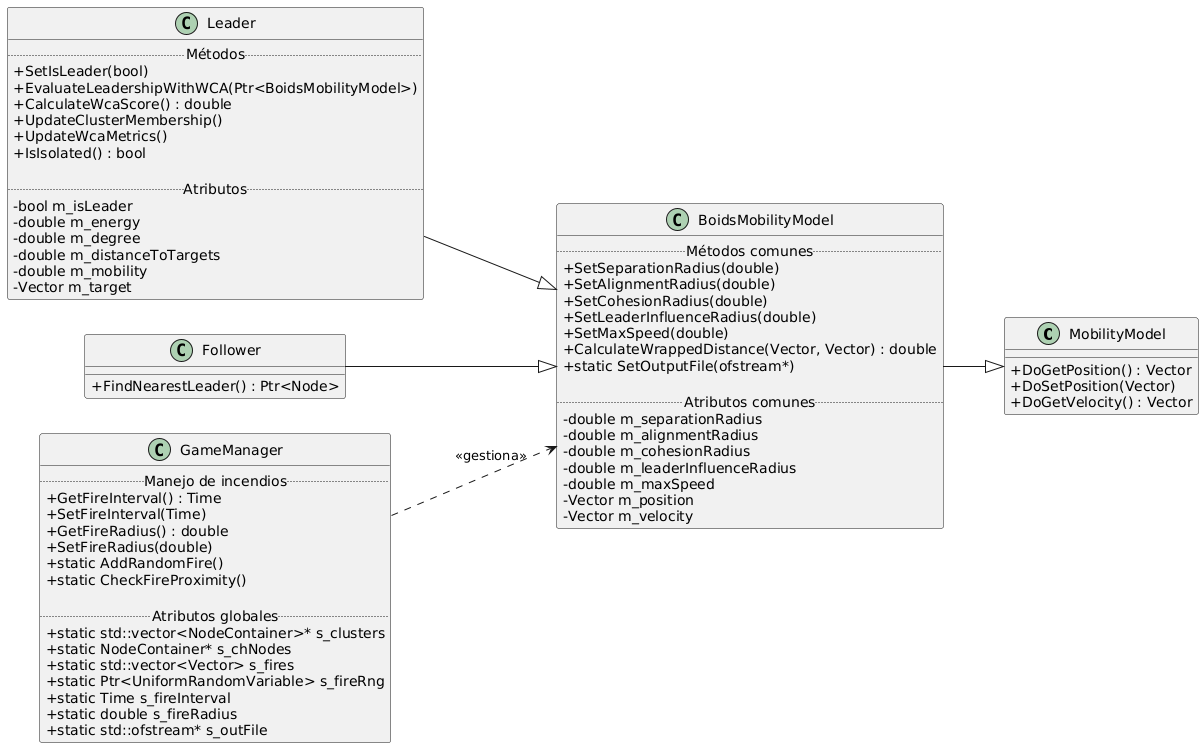
\includegraphics[width=0.9\textwidth]{class_diagram.png}
    \caption{Diagrama UML de la clase \texttt{BoidsMobilityModel}.}
    \label{fig:uml-boids}
\end{figure}

\section{Diagrama de Flujo de la Simulación}
El diagrama de flujo de la simulación ilustra el proceso general de la simulación, desde la inicialización de los nodos y su asignación de roles, hasta la actualización periódica de sus posiciones y la gestión de incendios. En cada iteración, los nodos evalúan su estado, actualizan sus posiciones según las reglas del modelo Boids, y determinan si deben asumir un rol de líder temporal en caso de estar aislados.
\begin{figure}[H]
    \centering
    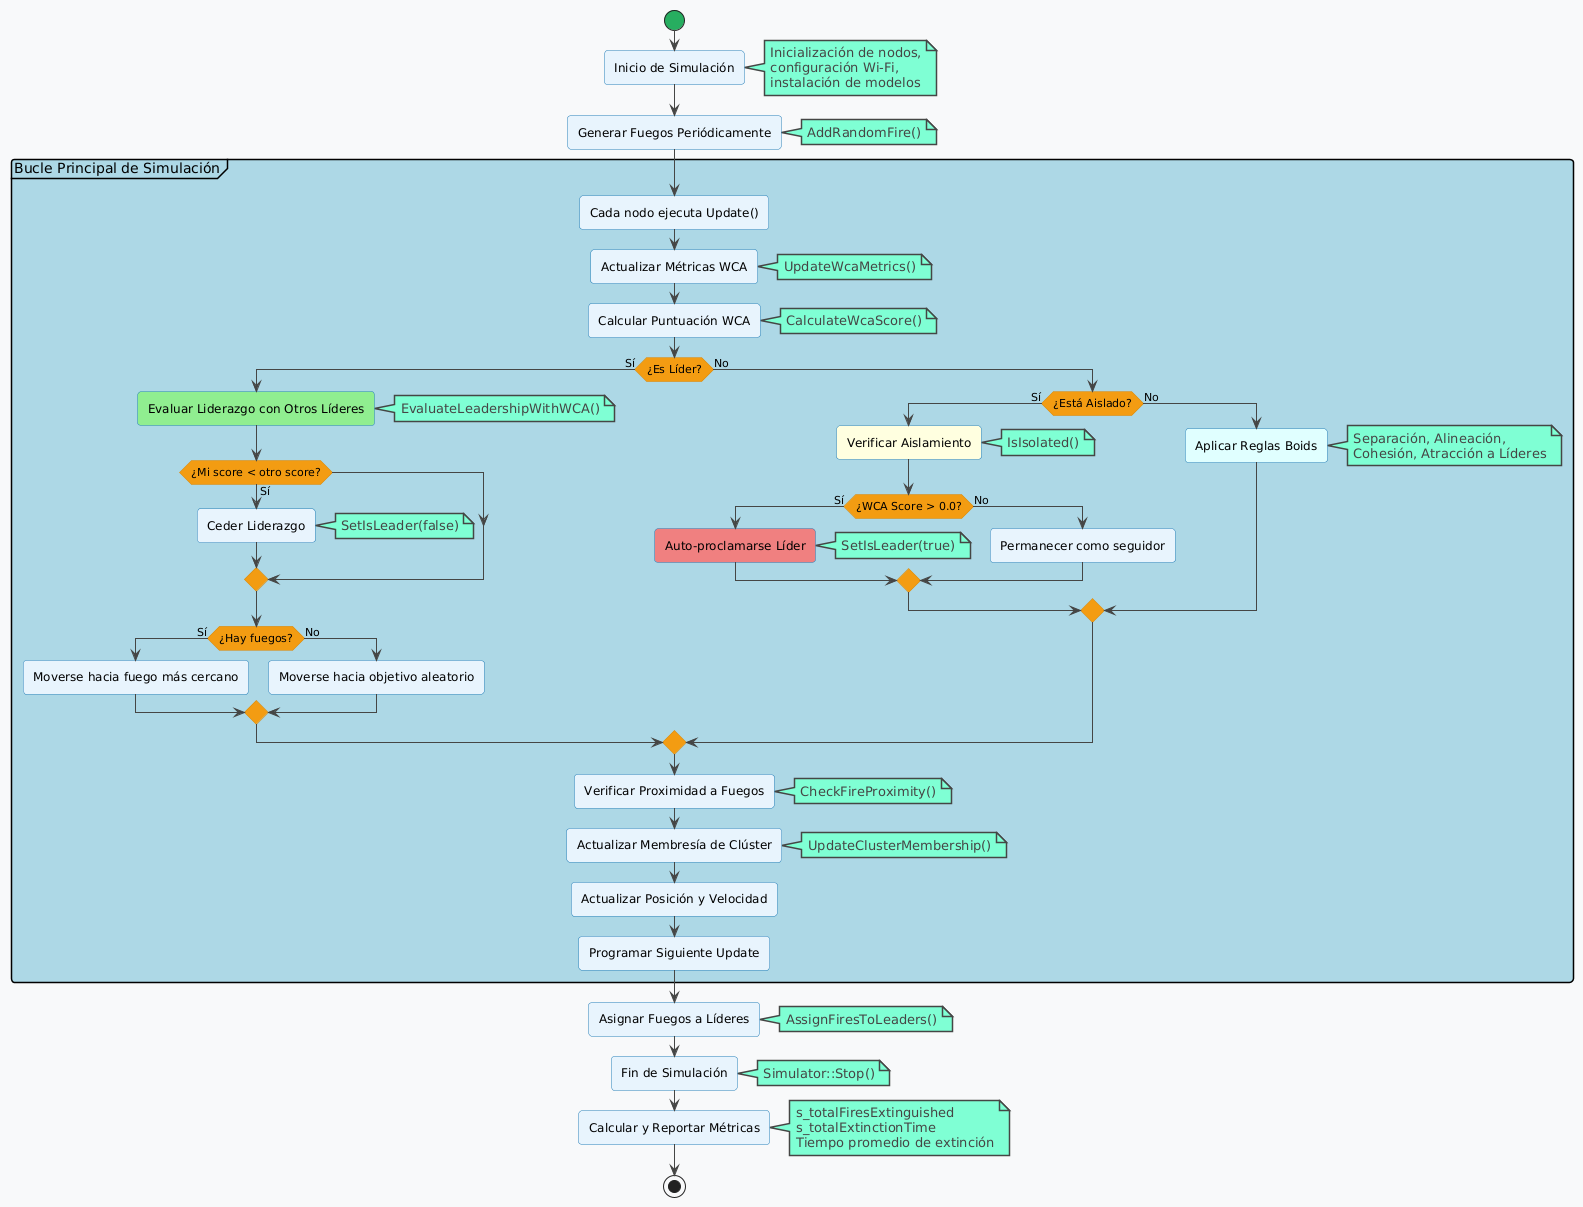
\includegraphics[width=1\textwidth]{flow_simulation_diagram.png}
    \caption{Diagrama de flujo de la simulación.}
    \label{fig:uml-flow}
\end{figure}

\section{Modelos Estocásticos y Distribuciones Empleadas en la Simulación de MANET para Extinción de Fuegos}

La simulación de Redes Ad Hoc Móviles (MANET) para la extinción de fuegos incorpora elementos de aleatoriedad para simular un comportamiento realista tanto en el entorno como en los nodos. Esto se logra mediante el empleo de diversos modelos estocásticos y distribuciones de probabilidad.

\subsection*{1. Generación de Fuegos: Proceso de Clúster de Thomas (Poisson Espacial)}
Los fuegos no aparecen de manera completamente aleatoria, sino que tienden a agruparse, lo cual se simula mediante un \textbf{proceso de clúster de Thomas} [1-4]. Este proceso consta de dos etapas principales:

\begin{itemize}
    \item \textbf{Generación de Centros de Clúster}: Se generan $k$ (por defecto 3 [4]) centros de clúster de forma uniforme dentro del área de simulación (1000x1000 unidades) [3].
    \begin{equation*}
        C_i.x \sim U(0, 1000) \quad \text{y} \quad C_i.y \sim U(0, 1000)
    \end{equation*}
    Donde $C_i$ representa el $i$-ésimo centro de clúster, y $U(a, b)$ denota una \textbf{distribución uniforme continua} en el intervalo $[a, b]$ [3].

    \item \textbf{Generación de Focos de Fuego Individuales}: Alrededor de cada centro $C_i$, se generan los focos de fuego individuales $F_j$. Sus posiciones se determinan añadiendo un desplazamiento aleatorio que sigue una \textbf{distribución normal (gaussiana)} [5-7].
    \begin{align*}
        F_j.x &= C_i.x + \delta_x \\
        F_j.y &= C_i.y + \delta_y
    \end{align*}
    Donde $\delta_x$ y $\delta_y$ son variables aleatorias muestreadas de una \textbf{distribución normal} con media cero y una varianza determinada por la desviación estándar:
    \begin{equation*}
        \delta_x \sim N(0, \text{desviacion}^2) \quad \text{y} \quad \delta_y \sim N(0, \text{desviacion}^2)
    \end{equation*}
    La \textbf{desviación estándar por defecto} para los fuegos es de \textbf{50.0 metros} [4]. Las coordenadas resultantes se recortan para asegurar que permanezcan dentro del área de simulación [6, 7].

    \item \textbf{Número de Fuegos por Evento}: Cada vez que se añade un nuevo evento de fuego, el número de fuegos generados es entre 1 y 3, determinado por una \textbf{variable aleatoria uniforme entera} [8].
    \begin{equation*}
        N_{\text{fuegos}} \sim U_{\text{entero}}(1, 3)
    \end{equation*}

    \item \textbf{Intervalo de Aparición de Fuegos}: Los nuevos fuegos aparecen en intervalos fijos.
    \begin{equation*}
        T_{\text{intervalo\_fuego}} = 8 \text{ segundos} [9, 10].
    \end{equation*}
\end{itemize}

\subsection*{2. Consumo de Energía de los Nodos}
La \textbf{energía} ($m\_energy$) de los nodos, una métrica clave para el cálculo del puntaje WCA, disminuye con el tiempo. El consumo se modela de forma simplificada, restando un valor muestreado de una \textbf{distribución normal} en cada actualización.
\begin{equation*}
    \Delta \text{Energía} \sim N(0.005, \sigma^2)
\end{equation*}
Donde la media de 0.005 representa el consumo promedio por unidad de tiempo. La varianza ($\sigma^2$) no se especifica directamente, pero es parte de la configuración del `NormalRandomVariable` utilizado [20]. El valor de energía se asegura que no sea negativo ($\max(0.0, \dots)$) [20].


\section{Código Fuente}\label{sec:cod}

El código fuente completo se encuentra adjunto como Taller1.zip
o en el siguiente repositorio de GitHub:

\begin{center}
\url{https://github.com/JavierTarazona06/ME01_Tareas/tree/main/Taller1/Code/boids}
\end{center}

\begin{table}[ht]
  \centering
  \begin{tabular}{p{4cm} p{10cm}}
    \toprule
    \textbf{Archivo} & \textbf{Función} \\
    \midrule
    \texttt{CMakeLists.txt} &
      - Instrucciones de construcción para compilar el proyecto.

      - Cómo integrar este módulo de movilidad (“mobility”) en la compilación de NS-3.

      - Define la librería \texttt{mobility}, lista los archivos fuente (incluyendo \texttt{boids-mobility-model.cc}), especifica dependencias (antenas, red) y registra los tests asociados.
    \\
    \addlinespace
    \texttt{boids-mobility-model.h} &
      - Declaración de la clase \texttt{BoidsMobilityModel}, que hereda de \texttt{ns3::MobilityModel}.

      - Parámetros configurables: radios de separación, alineamiento, cohesión y liderazgo; velocidad máxima; bandera de “líder”; intervalos de “fuego” (evento interno).

      - Método estático \texttt{SetOutputFile(\dots)} para indicar dónde volcar la trayectoria de los nodos.
    \\
    \addlinespace
    \texttt{boids-mobility-model.cc} &
      Implementación de la lógica Boids:

          - Cálculo de separación, alineamiento, cohesión y término de influencia de líderes.

          - Gestión de “fuegos” y escritura de posiciones en el archivo de salida.
    \\
    \addlinespace
    \texttt{boids.cc} &
    Script de simulación “usuario” que configura nodos, asigna el modelo \texttt{BoidsMobilityModel}, fija parámetros y ejecuta la simulación.
    \\
    \addlinespace
    \texttt{simulate/boids \_positions.csv} &
    Archivo generado por la simulación NS-3 (desde \texttt{boids.cc}) con un registro tabulado de tiempo, nodo y coordenadas (x, y, z, …).
    \\
    \addlinespace
    \texttt{simulate/showNodes.py} &
    Script en Python que carga el CSV con \texttt{pandas} y usa \texttt{matplotlib} para animar los movimientos de los nodos.
    \\
    \bottomrule
  \end{tabular}
  \caption{Descripción de los archivos del proyecto Boids en NS-3}
  \label{tab:boids_files}
\end{table}


\section{Manual Usuario}\label{sec:man_u}

%---------------------------------------------------------------------------------
% Manual Usuario ---------------------------------------------------------
%---------------------------------------------------------------------------------
Este manual guiará al usuario a través de los pasos necesarios para instalar NS-3 en un entorno WSL (Windows Subsystem for Linux), configurar los archivos para la simulación de boids y ejecutar dicha simulación, así como visualizar sus resultados.

\section*{\textbf{0. Prerequisitos}}

% Formato de la sección
Para seguir este manual, es necesario tener conocimientos básicos de Linux y C++. Además, se recomienda familiarizarse con el entorno de NS-3 y sus conceptos fundamentales.


Antes de comenzar, asegúrate de tener lo siguiente:
\begin{itemize}
    \item Conexión a Internet para descargar NS-3 y sus dependencias.
    \item Conocimientos básicos de terminal de Linux y C++.
    \item CMake y un compilador C++ (g++) instalados en tu sistema.
    \item WSL (Windows Subsystem for Linux) instalado en tu sistema Windows.
        \begin{itemize}
            \item Preferiblemente con una distribución de Linux como Ubuntu.
        \end{itemize}
    \item \textbf{Python 3} con los paquetes \textbf{pandas} y \textbf{matplotlib} instalados.
        \begin{itemize}
            \item De no tenerlos instalados, puedes hacerlo ejecutando:
            \begin{lstlisting}
pip3 install pandas matplotlib
            \end{lstlisting}
        \end{itemize}
\end{itemize}

\section*{\textbf{1. Instalación de NS-3 en WSL}}
Para instalar NS-3, se recomienda usar WSL, preferentemente con Ubuntu .

\begin{itemize}
    \item \textbf{Iniciar WSL}: Abre tu terminal WSL.
    \item \textbf{Actualizar Paquetes}: Ejecuta el siguiente comando para actualizar la lista de paquetes:
    \begin{lstlisting}
sudo apt update 
    \end{lstlisting}
    \item \textbf{Instalar Dependencias Esenciales}: Instala las herramientas de compilación y descompresión necesarias:
    \begin{lstlisting}
sudo apt install g++
sudo apt install bzip2
sudo apt install make 
sudo apt-get install cmake 
    \end{lstlisting}
    \item \textbf{Configurar Alias de Python}: NS-3 utiliza Python 3. Para asegurarte de que el comando \texttt{python} apunte a \texttt{python3}, añade un alias a tu archivo \texttt{.bashrc} y recarga la configuración:
    \begin{lstlisting}
echo alias python=python3 >> ~/.bashrc 
source ~/.bashrc 
    \end{lstlisting}
\end{itemize}

\section*{\textbf{2. Descarga y Preparación de NS-3}}

\begin{itemize}
    \item \textbf{Navegar a la Carpeta de Instalación}: Dentro de WSL, tu sistema de archivos de Windows se encuentra en \texttt{/mnt/c} (si tu partición es C:) o \texttt{/mnt/d} (si es D:). Navega a la carpeta donde deseas instalar NS-3. Por ejemplo:
    \begin{lstlisting}
cd /mnt/c/Users/TuUsuario/Documentos/NS3_Projects 
    \end{lstlisting}
    \item \textbf{Descargar NS-3}: Descarga el archivo \texttt{ns-allinone-3.45.tar.bz2} desde la página oficial de NS-3 (\url{https://www.nsnam.org/releases/ns-allinone-3.45.tar.bz2}) y guárdalo en la carpeta deseada. Es preferible hacerlo desde el navegador web de Windows y luego acceder a la ruta desde WSL.
    \item \textbf{Extraer Archivos}: Una vez descargado, descomprime el archivo tar.bz2:
    \begin{lstlisting}
tar xjf ns-allinone-3.45.tar.bz2
    \end{lstlisting}
    \textit{Nota: Aunque las fuentes mencionan \texttt{ns-3.45.tar.bz2} , el paso de descarga}

        \textit{sugiere \texttt{ns-allinone-3.45.tar.bz2}.}
    \item \textbf{Acceder al Directorio de NS-3}: Navega al directorio principal de NS-3:
    \begin{lstlisting}
cd ns-3.45  
    \end{lstlisting}
\end{itemize}

\section*{\textbf{3. Configuración y Compilación de NS-3}}

Desde el directorio \texttt{ns-3.45} (o la versión que estés usando), ejecuta los siguientes comandos:

\begin{itemize}
    \item \textbf{Limpiar Compilación (Opcional pero recomendado)}:
    \begin{lstlisting}
./ns3 clean 
    \end{lstlisting}
    \item \textbf{Configurar NS-3}: Este paso configura el entorno de compilación. Asegúrate de incluir las opciones para depuración, ejemplos, pruebas y NetAnim:
    \begin{lstlisting}
./ns3 configure \
--build-profile=debug \
--enable-examples \
--enable-tests \
--enable-build-version \
-- -DNS3_NETANIM=ON 
    \end{lstlisting}
    \item \textbf{Compilar NS-3}: Este comando compila todo el proyecto NS-3. Puedes usar la opción \texttt{-j\$(nproc)} para utilizar todos los procesadores de tu equipo y acelerar la compilación:
    \begin{lstlisting}
./ns3 build 
    \end{lstlisting}
    Alternativamente, para usar todos los procesadores:
    \begin{lstlisting}
./ns3 build -j$(nproc) 
    \end{lstlisting}
    \item \textbf{Verificar la Instalación (Opcional)}:
    \begin{itemize}
        \item Ejecutar pruebas: \texttt{./test.py} 
        \item Ejecutar un ejemplo básico: \texttt{./ns3 run first} 
        \item Mostrar la versión instalada: \texttt{./ns3 show version} 
    \end{itemize}
\end{itemize}

\section*{\textbf{4. Configuración y Ejecución de la Simulación de Boids}}

La simulación de boids implica modificar y añadir archivos al proyecto NS-3, de los ya presentes para una mayor simplicidad. Sin embargo tambien puedes crear links simbólicos a los archivos necesarios en el directorio \texttt{scratch} de NS-3. A continuación se detallan los pasos para configurar y ejecutar la simulación de boids:

\begin{itemize}
    \item \textbf{Crear el Archivo Principal del Proyecto (\texttt{boids.cc})}:
    \begin{itemize}
        \item Copia el archivo llamado \texttt{boids.cc} en el subdirectorio \texttt{scratch} de tu instalación NS-3. Por convención, se hace en \texttt{ns-allinone-3.45/ns-3.45/scratch} .
        \item El contenido de este archivo lo puedes encontrar en repositorio proporcionado anteriormente.
    \end{itemize}
    \item \textbf{Añadir Modelos de Movilidad}:
    \begin{itemize}
        \item Copia los archivos \textbf{\texttt{boids-mobility-model.cc}} y 
            \textbf{\texttt{boids-mobility-model.h}} 
            
            a la ruta \texttt{ns3.xx/src/mobility/model}.
        \item El contenido de \texttt{boids-mobility-model.cc} se encuentra en los extractos de "Modelo de Movilidad Boids con Liderazgo Adaptativo".
        \item El contenido de \texttt{boids-mobility-model.h} se encuentra en los extractos de "Modelo de Movilidad Boids para Redes Inalámbricas".
    \end{itemize}
    \item \textbf{Modificar \texttt{CMakeLists.txt}}:
    \begin{itemize}
        \item Debes modificar el archivo \texttt{ns3.xx/src/mobility/CMakeLists.txt}.
        \item Añade la línea \texttt{model/boids-mobility-model.cc} para que se compile.
    \end{itemize}
    \item \textbf{Recompilar NS-3}: Después de hacer estos cambios, necesitas volver a compilar NS-3 para que los nuevos archivos se integren:
    \begin{lstlisting}
./ns3 build 
    \end{lstlisting}
    O, para usar todos los procesadores:
    \begin{lstlisting}
./ns3 build -j$(nproc) 
    \end{lstlisting}
    \item \textbf{Ejecutar la Simulación de Boids}:
    \begin{itemize}
        \item Desde el directorio principal de NS-3 (\texttt{ns-3.43}), ejecuta tu proyecto de boids:
        \begin{lstlisting}
./ns3 run scratch/boids 
        \end{lstlisting}
        (Asumiendo que tu archivo se llama \texttt{boids.cc} en la carpeta \texttt{scratch}).
    \end{itemize}
\end{itemize}

\section*{\textbf{5. Parámetros y Salida de la Simulación de Boids}}

\begin{itemize}
    \item \textbf{Modificar Parámetros de la Simulación}:
    \begin{itemize}
        \item Puedes ajustar el número de líderes (Cluster-Heads) y miembros directamente en el archivo \texttt{boids.cc}.
        \item Busca las siguientes líneas y modifica los valores según necesites:
        \begin{lstlisting}[language=C++]
static const uint32_t N_CH = 2; // Cantidad de lideres (Cluster-Heads) 
static const uint32_t N_MEM = 25; // Cantidad de miembros (seguidores)
        \end{lstlisting}
        \textit{Recuerda recompilar después de modificar \texttt{boids.cc} para que los cambios surtan efecto.}
    \end{itemize}
    \item \textbf{Generación de Datos}:
    \begin{itemize}
        \item El programa \texttt{boids.cc} \textbf{genera un archivo \texttt{boids\_positions.csv}}.
        \item Este archivo contiene datos de tiempo, ID del nodo, coordenadas X e Y, si el nodo es líder (\texttt{IsLeader}), y si la entrada representa un fuego (\texttt{IsFire}).
    \end{itemize}
\end{itemize}

\section*{\textbf{6. Visualización de la Simulación}}

\begin{itemize}
    \item \textbf{Script de Visualización}:
    \begin{itemize}
        \item El archivo \texttt{boids\_positions.csv} se utiliza con el script de Python \textbf{\texttt{showNodes.py}} para visualizar la simulación.
        \item El script \texttt{showNodes.py} lee los datos del CSV y utiliza \texttt{matplotlib} para animar el movimiento de los boids y la aparición de fuegos.
    \end{itemize}
    \item \textbf{Características de \texttt{showNodes.py}}:
    \begin{itemize}
        \item \textbf{Boids}: Se dibujan como puntos, con \textbf{líderes en rojo y seguidores en azul}.
        \item \textbf{Fuegos}: Se dibujan como \textbf{triángulos amarillos} [72].
        \item \textbf{Zonas de Influencia de Líderes}: Se representan como círculos rojos con transparencia alrededor de los líderes, con un radio de 100.
        \item \textbf{Controles de Visibilidad}: Puedes activar o desactivar la visualización de fuegos y zonas de líderes mediante botones interactivos.
    \end{itemize}
    \item \textbf{Ejecutar la Visualización}:
    \begin{itemize}
        \item Asegúrate de que \texttt{showNodes.py} esté en la misma carpeta que \texttt{boids\_positions.csv}.
        \item Ejecuta el script de Python: \texttt{python showNodes.py}
    \end{itemize}
\end{itemize}

%---------------------------------------------------------------------------------
% Manual Técnico ---------------------------------------------------------
%---------------------------------------------------------------------------------

\section*{Descripción del Proceso de Elección de Líderes y Propuesta de Mejora en MANETs}

Para comprender la dinámica de liderazgo en nuestra simulación de \textbf{Redes Ad Hoc Móviles (MANET)}, es fundamental distinguir entre la configuración base y la mejora propuesta en nuestra \textbf{Indagación al Estilo Newtoniano}.

\subsection*{Elección de Líderes en el Escenario Base (Condición de Control)}

En la configuración inicial, la elección y gestión de líderes se rige por un \textbf{esquema de liderazgo adaptativo} que emplea el \textbf{algoritmo WCA (Weighted Cluster Algorithm)}. Los nodos en la MANET exhiben un \textbf{modelo de movilidad tipo Boids}, lo que significa que sus movimientos se inspiran en el comportamiento de bandadas, cardúmenes o enjambres, regulados por reglas de separación, alineación y cohesión.

Los \textbf{líderes, o \texttt{chNodes}}, son los designados para la tarea crucial de \textbf{extinguir fuegos (\texttt{s\_fires})} que aparecen aleatoriamente en el entorno de simulación.

El \textbf{puntaje WCA} de un nodo es un indicador de su idoneidad para ser líder, y se calcula ponderando cuatro métricas normalizadas:

\begin{itemize}
  \item \textbf{Energía (\texttt{m\_energy})}: Representa la energía residual del nodo, normalizada en el rango.
  \item \textbf{Grado de Conectividad (\texttt{m\_degree})}: Mide el número de vecinos dentro del radio de influencia del líder (\texttt{m\_leaderInfluenceRadius}), normalizado asumiendo un máximo teórico de 10 vecinos.
  \item \textbf{Distancia a Objetivos (\texttt{m\_distanceToTargets})}: Cuantifica la distancia promedio a los fuegos activos, normalizada inversamente (mayor cercanía = mayor puntuación) considerando un radio de 200m.
  \item \textbf{Movilidad (\texttt{m\_mobility})}: Refleja la estabilidad del nodo (baja movilidad = mayor puntuación), normalizada inversamente asumiendo una velocidad máxima de 10 m/s.
\end{itemize}

Los \textbf{pesos asignados} a estas métricas en la fórmula WCA son:

\begin{itemize}
  \item Energía (\texttt{w1}): 0.4
  \item Grado de Conectividad (\texttt{w2}): 0.3
  \item Proximidad a Objetivos (\texttt{w3}): 0.2
  \item Estabilidad (baja movilidad) (\texttt{w4}): 0.1
\end{itemize}

Así, el \texttt{wcaScore} se calcula como:

\begin{center}
\texttt{(w1 * normEnergy) + (w2 * normDegree) + (w3 * normTargetDistance) + (w4 * normMobility)}
\end{center}

El resultado final se ajusta para estar entre 0.0 y 1.0.

En esta condición de control, los nodos \textbf{se inicializan explícitamente como líderes (\texttt{chNodes}) o seguidores (\texttt{memberNodes})}. Los \textbf{líderes existentes} evalúan continuamente su liderazgo con otros líderes cercanos utilizando el algoritmo WCA. Si un líder (\texttt{m\_isLeader} es verdadero) se encuentra con otro líder dentro de su radio de influencia (\texttt{m\_leaderInfluenceRadius}) y este último posee un puntaje WCA superior, el líder con la puntuación inferior puede \textbf{ceder su rol} (\texttt{SetIsLeader(false)}).

Por otro lado, los \textbf{nodos seguidores} (\texttt{!m\_isLeader}) se comportan conforme a las reglas de Boids (separación, alineación, cohesión) y son atraídos hacia los líderes dentro de su radio de influencia. Su función principal es unirse a un clúster liderado por el líder más cercano.

En este escenario base, la sección de código que permite la autopromoción de un seguidor a líder se encuentra \textbf{desactivada o eliminada}, lo que significa que un nodo inicialmente seguidor \textbf{no puede autonombrarse líder} bajo ninguna circunstancia.

\subsection*{Introducción de la Propuesta: Autopromoción de Nodos Seguidores}

La \textbf{Indagación al Estilo Newtoniano propuesta} plantea la siguiente hipótesis central:

\begin{quote}
"¿No será que la \textbf{efectividad global en la extinción de fuegos} (medida por métricas como el tiempo promedio de extinción, el número total de fuegos extinguidos en un periodo dado) \textbf{se incrementa} si se permite que un nodo seguidor que previamente estaba \textbf{aislado} (sin un líder cercano dentro de un radio efectivo de influencia) \textbf{se autoproclame temporalmente como líder hasta que se encuentre con uno con un mayor WCA}?"
\end{quote}

Para probar esta hipótesis, se introduce una \textbf{funcionalidad clave} en la Condición Experimental que modifica el comportamiento de los nodos seguidores. Un nodo seguidor (\texttt{!m\_isLeader}) ahora tiene la capacidad de \textbf{autoproclamarse temporalmente como líder} si cumple las siguientes condiciones, evaluadas en cada ciclo de \texttt{Update()}:

\begin{enumerate}
  \item \textbf{No es un líder actual} (\texttt{!m\_isLeader}).
  \item Se encuentra \textbf{aislado} (\texttt{IsIsolated()}), es decir, sin líderes dentro de un \textbf{radio de influencia efectivo ampliado} (\texttt{m\_leaderInfluenceRadius * 1.2}).
  \item Posee un \textbf{puntaje WCA (\texttt{wcaScore}) superior a 0.0}.
\end{enumerate}

Si cumple estas condiciones, se le asigna el rol de líder (\texttt{SetIsLeader(true)}), se le designa un \textbf{objetivo aleatorio} (\texttt{m\_target}) dentro del área de simulación (0--1000 en X e Y), y su \textbf{velocidad (\texttt{m\_velocity}) se incrementa ligeramente (x1.05)} para facilitar su búsqueda de fuegos.

Al igual que los líderes iniciales, los nodos autopromovidos siguen participando en el mecanismo de evaluación de liderazgo del WCA. Si se encuentran con un líder con mayor puntaje, pueden \textbf{ceder su rol} y volver a ser seguidores.

\subsection*{Escenarios de Experimentación}

Para evaluar el impacto de esta propuesta, se comparan los resultados de la \textbf{Condición de Control} y la \textbf{Condición Experimental (Hipótesis Propuesta)} bajo diferentes configuraciones del número de nodos seguidores. La \textbf{efectividad global en la extinción de fuegos} se mide mediante el \textbf{número total de fuegos extinguidos} y el \textbf{tiempo promedio de extinción}.

\textbf{Parámetros Comunes para Todos los Escenarios}:

\begin{itemize}
  \item \textbf{Número de Líderes Iniciales (\texttt{N Clusters})}: 2
  \item \textbf{Área de Simulación}: 1000x1000 unidades
  \item \textbf{Radio de Detección de Fuego (\texttt{s\_fireRadius})}: 30.0 metros
  \item \textbf{Intervalo de Aparición de Fuegos (\texttt{s\_fireInterval})}: Cada 8 segundos (1 a 3 fuegos por evento, distribución tipo clúster de Thomas)
  \item \textbf{Velocidad Máxima de Líderes}: 6.5 m/s
  \item \textbf{Velocidad Máxima de Seguidores}: 6.0 m/s
  \item \textbf{Duración de la Simulación}: 100 segundos
\end{itemize}

La variación del \textbf{número de seguidores (\texttt{N Members})} es esencial para analizar la robustez y escalabilidad del sistema bajo distintas densidades.

\begin{table}[H]
\centering
\caption{Resultados de la Simulación por Escenario y Condición}
\label{tab:results}
\begin{tabular}{llccc}
\toprule
\textbf{Escenario} & \textbf{N. de Seguidores} & \textbf{Condición} & \textbf{Fuegos Apagados} & \textbf{Tiempo Promedio (s)} \\
\midrule
1 & 10 & Control      & 15 & 8.67  \\
  &    & Experimental & 16 & 11.38 \\
\midrule
2 & 15 & Control      & 12 & 17.33 \\
  &    & Experimental & 17 & 17.50 \\
\midrule
3 & 25 & Control      & 11 & 11.88 \\
  &    & Experimental & 16 & 7.81  \\
\bottomrule
\end{tabular}
\end{table}



\section{Experimentación}\label{sec:exp}

\subsection{Documentación}


\subsection{Escenario 1:}


\subsection{Escenario 2:}

\subsection{Escenario 3:}

\subsection{Comparación resultados}

%---------------------------------------------------------------------------------
% Conclusiones ---------------------------------------------------------
%---------------------------------------------------------------------------------

\section{Conclusiones}\label{sec:concl}

La integración del modelo Boids permite simular comportamientos realistas en redes móviles
El uso del modelo Boids reproduce dinámicas naturales de agrupamiento, separación y alineación, lo cual resulta útil para representar redes MANET (redes móviles ad hoc) en situaciones como búsqueda, exploración o evacuación.
%---------------------------------------------------------------------------------
% Recomendaciones ---------------------------------------------------------
%---------------------------------------------------------------------------------

\section{Recomendaciones}\label{secrecomen}

Aunque el movimiento fue simulado correctamente, se recomienda analizar también cómo este afecta la calidad de las comunicaciones (ej. transmisión de datos entre nodos), especialmente al estar en constante movimiento y ante interrupciones externas.

\section{Referencias}
\renewcommand{\refname}{}
\begin{thebibliography}{9}

\bibitem{ref} \label{ref:AdHoc} S. K. Sarkar, T. G. Basavaraju y C. Puttamadappa, 
Ad Hoc Mobile Wireless Networks: Principles, Protocols, and Applications, 2ª ed. 
Boca Raton, FL: CRC Press, 2013.

\bibitem{ref} \label{ref:PrinciplesAdHoc} M. Barbeau y E. Kranakis, Principles of Ad Hoc 
Networking, 1ª ed. Chichester, England; Hoboken, NJ: Wiley, May 2007.

\end{thebibliography}

\end{document}